\documentclass[t,10pt,mathserif,xcolor=pst,pdftex]{beamer}
\mode<presentation>

\usetheme{Berkeley}
\usecolortheme{dolphin}
\beamertemplatenavigationsymbolsempty
\usefonttheme[onlylarge]{serif}
\usepackage[version=4]{mhchem}

\usepackage[USenglish]{babel}
\usepackage[utf8]{inputenc}
\usepackage[T1]{fontenc}
\usepackage{colortbl}
\usepackage{pstricks}
\usepackage{multimedia}
\usepackage{bm}
\usepackage{nicefrac}
\usepackage{charter}
\newcommand{\be}{\begin{equation}} 
\newcommand{\ee}{\end{equation}}  
\newcommand{\pd}{\partial}

\title[Chem 132A]{Physical Chemistry (Chem 132A)}

\author[Shane Flynn]{Presentation By: Shane Flynn}
\institute[UC Irvine]{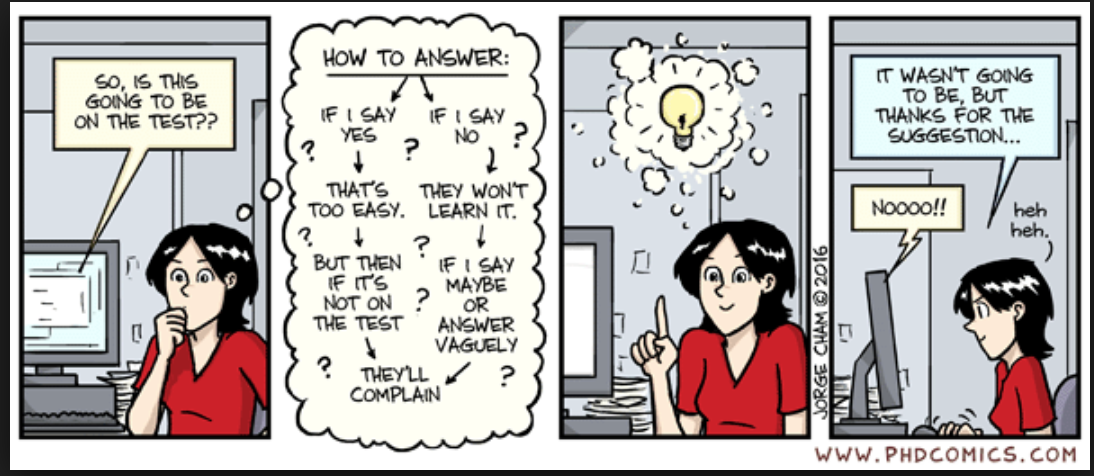
\includegraphics[height=0.40\textheight,width=0.7\textwidth]{phd.png}\\[1mm]
Department of Chemistry, University of California, Irvine, 2208 Natural Sciences II}

\date\today

\pgfdeclareimage[height=1.5cm]{logo}{uc_seal.png}
\logo{\pgfuseimage{logo}}

\begin{document}

\begin{frame}
\titlepage
\end{frame}

\section{Exam Overview}

\subsection{Logistics}

\begin{frame}{Exam Wednesday (10/25/17)!}
\begin{itemize}
\item 45 Minute Exam
\end{itemize}

\begin{itemize}
\item Try to be here at 10:50am
\end{itemize}

\begin{itemize}
\item Bring your I.D. and Sit in YOUR seat!
\end{itemize}

\begin{itemize}
\item Do not bring excess 'stuff' to the exam.
\end{itemize}

\begin{itemize}
\item Questions, Comments, Concerns, Raise your hand!
\end{itemize}

\begin{itemize}
\item You CANNOT leave early!
\end{itemize}

\begin{itemize}
\item Bring a calculator (nothing that can access internet, etc). 
\end{itemize}

One 8.5 by 11 (in.) piece of paper with HAND-WRITTEN notes (equations and text). 
You can use both sides of the paper and write whatever you want!

\end{frame}

\begin{frame}{Everything is on the Exam}

\begin{itemize}
\item Yes! You should read the book.
\end{itemize}

\begin{itemize}
\item Yes! The lecture material is on the exam.
\end{itemize}

\begin{itemize}
\item Yes! The Webassign is on the exam.
\end{itemize}

\begin{itemize}
\item Yes! The discussion problems are on the exam.
\end{itemize}

\begin{itemize}
\item Yes! Everything covered in Chapters 2, 3, and 4, or topics from discussion and lecture are on the exam. 
\end{itemize}

\begin{itemize}
\item STOP! Asking what you should study... I do not know you!
\end{itemize}

\begin{itemize}
\item Stop! Asking for our office/office hours (until after the exam)!
\end{itemize}

\begin{itemize}
\item Consider looking at the Github!
\end{itemize}

\end{frame}


\subsection{Material Summary}

\begin{frame}{The Story So Far}

\begin{itemize}
\item Terms: Reversible, Adiabatic, Isochoric, Open, ..... 
\end{itemize}

\begin{itemize}
\item The Laws of Thermodynamics
\end{itemize}
The First Law, The Second Law, and The Third Law.

\begin{itemize}
\item Thermodynamic Potentials
\end{itemize}
Internal Energy, Enthalpy, Helmholtz, Gibbs.

\begin{itemize}
\item State Functions, Path Functions, Equations of State. 
\end{itemize}

\begin{itemize}
\item Total Differentials and Partial Derivatives. 
\end{itemize}
Heat Capacity, Expansion Coefficient, Joule-Thomson Coefficient. 

\begin{itemize}
\item Deviations from Perfect (Ideal) Behavior. 
\end{itemize}

\end{frame}

\begin{frame}{The Story So Far (Part 2)}

\textbf{Gibbs Free Energy:}
\begin{itemize}
\item Characteristic variables: G(T,P)
\item As a function of Temperature only $\Rightarrow$ Gibbs-Helmholtz Equation. 
\item As a function of Pressure only $\Rightarrow$ fugacity. 
\item Chemical Potential!
\end{itemize}

\textbf{Phases:}
\begin{itemize}
\item $\mu$ $\equiv$ G$_m$ (single component system). 
\item Phase Diagrams!
\item solid, liquid, gas, supercritical fluid, triple point, phase line. 
\item Phase Rule 
\item First Order Phase Transition
\item Second Order Phase Transition
\end{itemize}

\begin{itemize}
\item Clapeyron equation ($\mu(\alpha)$ = $\mu(\beta)$)
\end{itemize}


\end{frame}

\subsection{Post-Exam}

\begin{frame}{Relax!}

\begin{itemize}
\item Feel Free to attend discussion Tuesday. Come ready to discuss, bring conceptual questions!
\end{itemize}

\\~\

\begin{itemize}
\item No Discussion Wednesday!
\end{itemize}

\\~\

\begin{itemize}
\item Thursday and Friday discussions will review the exam. 
\end{itemize}

\\~\

\begin{itemize}
\item Wait until we report back on grades before panicking. 
\end{itemize}

\\~\

\begin{itemize}
\item Come speak to the TAs or Professor Hemminger before taking 'drastic measures'. 
\end{itemize}

\end{frame}

\section{Examples}

\subsection{Themochemistry}

\begin{frame}{Enthalpy }

Consider the following chemical reaction. 
\be
\ce{CH4(g) + O2(g) <--> CO2(g) + H2O(l)}
\ee
Calculate the Enthalpy of Reaction for this reaction using standard Enthalpy of Formation values from the book. \\~\

\textbf{SOLUTION:}
Start by Balancing The Equation!
\be
\ce{CH4(g) + 2O2(g) <--> CO2(g) + 2H2O(l)}
\ee

Now \textbf{Algebraically} solve the question. 
\be
\Delta H_{\text{rxn}}^0[298] = 
\ee
\be
\Delta H_f^0(\ce{CO2_{,g}}) + \Delta 2H_f^0(\ce{H2O_{,l}}) - \Delta H_f^0(\ce{CH4_{,g}}) - \Delta 2H_f^0(\ce{O2_{,g}}) 
\ee

\be
\Delta H_{\text{rxn}}^0[298] = -890.36 \quad \text{kJ}/\text{mol}
\ee

\end{frame}

\subsection{Free Expansion}


\begin{frame}{Entropy}

Consider the free expansion of one mole of a perfect gas that doubles its volume. 
Accounting for PV work only, determine the change in Internal Energy, work, heat, and Entropy for this process. 

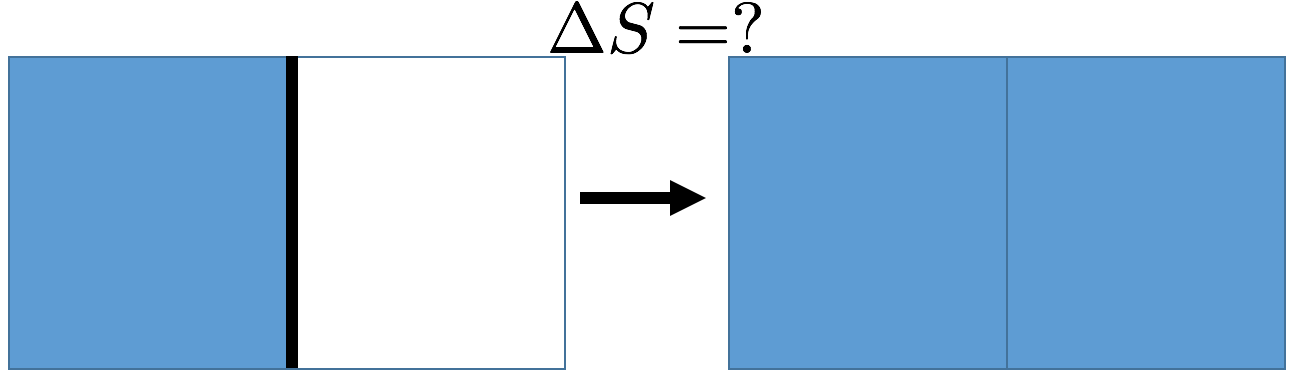
\includegraphics[height=0.40\textheight,width=1.0\textwidth]{gas.png}

\end{frame}

\begin{frame}{Entropy Solution:}
\begin{itemize}
\item $\Delta U$
\end{itemize}
\be
U(T), \Rightarrow \Delta U = 0
\ee

\begin{itemize}
\item w
\end{itemize}
w = 0, by definition of Free Expansion.

\begin{itemize}
\item q
\end{itemize}
\be
\Delta U = q + w \Rightarrow q = 0
\ee

\begin{itemize}
\item $\Delta S$
\end{itemize}
\be
S = \frac{q_r}{T}
\ee

\end{frame}

\begin{frame}{Entropy Solution (Part 2):}
Consider: A reversible isothermal expansion, from V$_1$ to V$_2$. 
\be
U = q + w, \Rightarrow q = -w
\ee

\begin{align*}
w = \int_{V_1}^{V_2} - P_{\text{ext}}dV\\
w = \int_{V_1}^{V_2} - P_{\text{g}}dV\\
w = -nRT \int_{V_1}^{V_2} \frac{dV}{V}\\
w = -RT\ln(2)
\end{align*}

\begin{align}
\Delta S_{\text{univ}} = \Delta S + \Delta S_{\text{surr}}\\
\Delta S_{\text{univ}} = \Delta S = R\ln(2) > 0
\end{align}

\end{frame}

\subsection{Phase Diagram}

\begin{frame}{Sulfur}

\begin{itemize}
\item Describe the Phase Diagram of Sulfur provided below (be sure to assign each letter). 
\end{itemize}

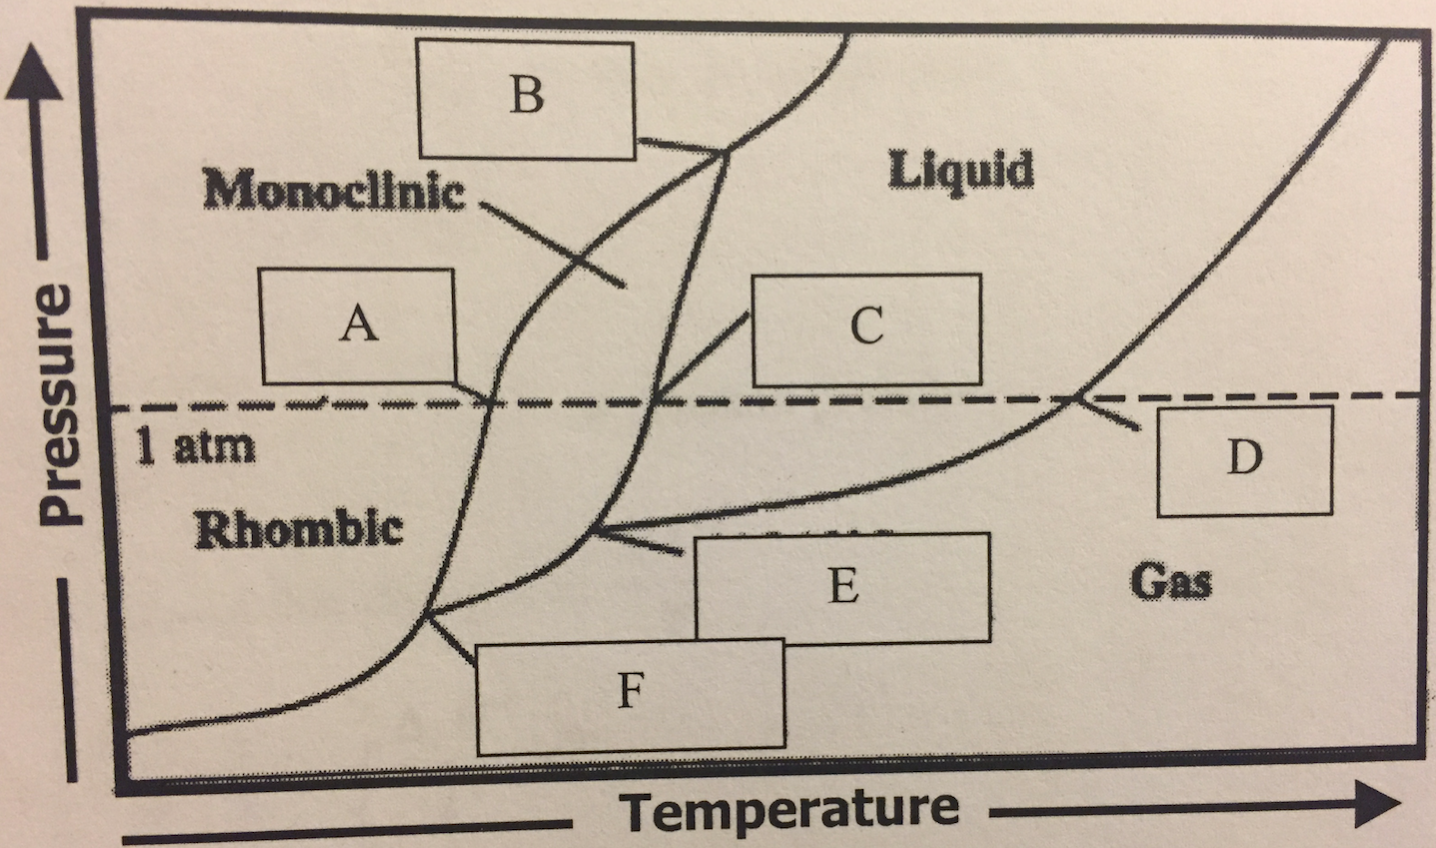
\includegraphics[height=0.70\textheight,width=.9\textwidth]{pd.png}

\end{frame}

\begin{frame}{Sulfur Solution:}
\textbf{Phases:}\\~\
P-T Phase Diagram with: two solid phases (rhombic, monoclinic), a liquid, and a gas phase (would assume if we keep heating we could get supercritical, but not on graph). \\~\

\textbf{Triple Points:}
\begin{itemize}
\item F: \quad $\mu_{\text{rhombic}}$ = $\mu_{\text{monoclinic}}$ = $\mu_{\text{gas}}$
\item E: \quad $\mu_{\text{liquid}}$ = $\mu_{\text{monoclinic}}$ = $\mu_{\text{gas}}$
\item B: \quad $\mu_{\text{rhombic}}$ = $\mu_{\text{monoclinic}}$ = $\mu_{\text{liquid}}$
\end{itemize}

\textbf{Transition Points:}
\begin{itemize}
\item A: \quad $\mu_{\text{rhombic}}$ = $\mu_{\text{monoclinic}}$ 
\item C: \quad $\mu_{\text{monoclinic}}$ = $\mu_{\text{liquid}}$
\item D: \quad $\mu_{\text{liquid}}$ = $\mu_{\text{gas}}$
\end{itemize}

Will an increase in Pressure raise or lower the melting point of sulfur? \qquad Raise!

\end{frame}

\section{Conclusion}

\begin{frame}{Summary}

\begin{itemize}
\item Read/Understand the book (hint try Google). 
\end{itemize}
\\~\

\begin{itemize}
\item Try the Discussion Problems (don't use solutions as a crutch). 
\end{itemize}
\\~\

\begin{itemize}
\item Look at Webassign (maybe focus on interesting problems). 
\end{itemize}
\\~\

\begin{itemize}
\item Look online or other books for inspiration. 
\end{itemize}
\\~\

\begin{itemize}
\item Make your 'cheat sheet'!
\end{itemize}
\\~\

\begin{itemize}
\item Learn where your seat is!
\end{itemize}

\end{frame}

\end{document}